\documentclass[10pt,conference]{IEEEtran}

\usepackage{amsmath}
\usepackage{amssymb}
\usepackage{graphicx}
\usepackage{booktabs}
\usepackage{xcolor}
\usepackage{hyperref}

% Quick visual marker for things that still need YOUR input (values,
% justification, discussion). Search for "todo" before submitting and
% make sure none are left.
\newcommand{\todo}[1]{\textcolor{red}{[TODO: #1]}}

\title{TMR4240 Marine Control Systems I\\
Project Part 1: Design of a Dynamic Positioning System}
\author{\IEEEauthorblockN{Group 7}
\IEEEauthorblockA{Department of Marine Technology, NTNU\\
Ivan Mordovets and Bastien Moreaux}}

\begin{document}
\maketitle

\begin{abstract}
\todo{Write the abstract last, once the results and conclusion exist.
One paragraph: what was built (3-DOF DP system for R/V Gunnerus in
Python), what was tested (station keeping, rotating current, setpoint
change, four-corner test), and the headline result.}
\end{abstract}

\section{Introduction}

Dynamic positioning (DP) systems automatically maintain a vessel's
position and heading using active thrusters rather than mooring lines
or anchors, compensating for environmental disturbances such as wind,
current, and waves \cite{fossen2011}. This report documents the design,
implementation, and validation of a basic three-degree-of-freedom (3-DOF)
DP system for the research vessel R/V Gunnerus, developed as Project
Part 1 of TMR4240 Marine Control Systems I.

The implemented system consists of five interconnected subsystems: a
current load model, a wind load model, a DP controller, a reference
model, and a thrust allocation algorithm. These subsystems interface
with a supplied three-DOF process plant model of R/V Gunnerus and a
simulation engine that handles state integration, actuator limits, and
logging.

\todo{One or two sentences on the report structure / roadmap, e.g.
``Section II introduces notation and coordinate frames... Section VI
presents the four mandatory simulations...''. Adjust section numbers
once the whole report is assembled.}

\section{Coordinate Frames and Notation}
\label{sec:frames}

\subsection{Coordinate Frames}

Two coordinate frames are used to describe the vessel motion. The
Earth-fixed North-East-Down (NED) frame, denoted $\{n\}$, is fixed to
the Earth with axes $x_n$ pointing North, $y_n$ pointing East, and
$z_n$ pointing Down. This frame describes the vessel's position and
heading relative to its surroundings.

The body-fixed frame, denoted $\{b\}$, is attached to the vessel, with
its origin at the vessel's centre of gravity. The $x_b$ axis points
forward toward the bow (surge), the $y_b$ axis points to starboard
(sway), and the $z_b$ axis points downward.

Both frames are right-handed. With the NED convention, a positive
rotation about the downward $z$ axis is clockwise when viewed from
above; consequently, the heading angle $\psi$ is measured clockwise
from North to the vessel's bow direction.

\todo{Insert your own version of the NED/body frame figure here
(Fig.~1 in the assignment PDF is a template for the idea only --
the report requires an original figure).}

\subsection{Six-DOF Notation and Three-DOF Reduction}

The standard six-DOF marine craft state vectors are
\begin{align}
\eta_6 &= [x,\, y,\, z,\, \phi,\, \theta,\, \psi]^\top, \\
\nu_6 &= [u,\, v,\, w,\, p,\, q,\, r]^\top, \\
\tau_6 &= [X,\, Y,\, Z,\, K,\, M,\, N]^\top.
\end{align}

Table~\ref{tab:notation} defines every component of these vectors and
the frame in which each is expressed.

\begin{table}[htbp]
\centering
\caption{Six-DOF notation}
\label{tab:notation}
\begin{tabular}{@{}clc@{}}
\toprule
Symbol & Description & Frame \\
\midrule
$x, y, z$ & Position (North, East, Down) & NED \\
$\phi, \theta, \psi$ & Roll, pitch, yaw (heading) & NED \\
$u, v, w$ & Surge, sway, heave velocity & Body \\
$p, q, r$ & Roll, pitch, yaw rate & Body \\
$X, Y, Z$ & Surge, sway, heave force & Body \\
$K, M, N$ & Roll, pitch, yaw moment & Body \\
\bottomrule
\end{tabular}
\end{table}

This project uses a horizontal-plane three-DOF model. Heave, roll,
and pitch are neglected; only surge, sway, and yaw are retained:
\begin{equation}
\eta = [N, E, \psi]^\top, \quad
\nu = [u, v, r]^\top, \quad
\tau = [X, Y, N_z]^\top,
\end{equation}
where $\eta$ is expressed in the NED frame and $\nu$, $\tau$ are
expressed in the body frame. This distinction between frames is
essential throughout the report: the vessel dynamics compute
accelerations in body axes, while position is integrated in the NED
frame.

\subsection{Kinematic Equation}

The kinematic equation converts body-frame velocity to NED position
and heading rates. It is a purely geometric transformation, not a
force model. For the three-DOF case it reduces to a yaw-only rotation:
\begin{equation}
\dot\eta = J(\psi)\,\nu, \qquad
J(\psi) = \begin{bmatrix}
\cos\psi & -\sin\psi & 0 \\
\sin\psi & \cos\psi & 0 \\
0 & 0 & 1
\end{bmatrix}.
\label{eq:kinematics}
\end{equation}

In scalar form,
\begin{equation}
\dot N = u\cos\psi - v\sin\psi, \quad
\dot E = u\sin\psi + v\cos\psi, \quad
\dot\psi = r.
\end{equation}

For this three-DOF rotation, $J^\top(\psi) = J^{-1}(\psi)$, so the
transpose can be used to convert NED-frame vectors (e.g.\ a position
error) into the body frame (e.g.\ a force direction). Heading errors
must always be wrapped to $(-\pi, \pi]$ using
\begin{equation}
\mathrm{wrap}(\alpha) = \operatorname{atan2}(\sin\alpha, \cos\alpha).
\label{eq:wrap}
\end{equation}

\section{Current Model}
\label{sec:current}

\emph{Note: the group member originally responsible for the current
model left the group, and the current model was therefore written
entirely by an AI assistant (Google, Gemini).}

The ocean current is defined in the NED frame by a speed
$V_c$ and a direction, using only the North and East components (the
vertical component is always zero). The direction input $\beta_c$
(0 = North, $\pi/2$ = East) is used with the ``from'' convention: the
water flows towards $\beta_c+\pi$, so
$V_{c,N}=V_c\cos(\beta_c+\pi)$ and $V_{c,E}=V_c\sin(\beta_c+\pi)$.
For example, ``current from east'' gives $V_{c,E}=-V_c$, i.e.\ water
flowing westward.

To act on the vessel, the current is transformed from the NED frame to
the body frame and subtracted from the vessel velocity to obtain the
relative velocity used by the plant model:
\begin{equation}
\nu_c^n = [V_{c,N},\, V_{c,E},\, 0]^\top, \qquad
\nu_c^b = J^\top(\psi)\,\nu_c^n, \qquad
\nu_r = \nu - \nu_c^b.
\label{eq:current}
\end{equation}

The current does not enter the vessel model as a separate generalised
force; instead it acts entirely through the relative velocity
$\nu_r$ inside the hydrodynamic damping terms. This means the current
model's only responsibility is to produce a correct NED velocity
vector $[V_{c,N}(t), V_{c,E}(t)]$ at each time step.

The current has constant speed and a direction that is either fixed
or rotated linearly in time,
$\beta_c(t)=\beta_0+\min(t/T_r,1)\,(\beta_1-\beta_0)$. Simulation~1a
uses $V_c=0.5$ m/s from east ($\beta_c=\pi/2$, fixed). Simulation~2
uses $V_c=0.5$ m/s with $\beta_c$ rotating from $0$ (north) to
$\pi/2$ (east) over $T_r=300$ s, as specified by the mandatory tests;
the speed stays constant while only the direction changes.

\section{Wind Model}
\label{sec:wind}

\emph{Note: the group member originally responsible for the wind
model left the group, and the wind model was therefore written
entirely by an AI assistant (Google, Gemini).}

The wind model returns a six-component generalised body-frame load
vector, of which only the surge, sway, and yaw entries
($\tau_{\mathrm{wind}}[0,1,5]$) affect the three-DOF plant. The wind
load is computed from the \emph{relative} wind speed and angle using a
tabulated coefficient vector:
\begin{equation}
\tau_{\mathrm{wind}} = U_{rw}^2\, C_w(\alpha_{rw}),
\label{eq:wind}
\end{equation}
where $C_w(\alpha_{rw}) \in \mathbb{R}^6$ is interpolated from the
supplied wind coefficient table (generated with the method of
Blendermann \cite{blendermann1994} for R/V Gunnerus; only $C_x$,
$C_y$, $C_\psi$ are non-zero for the horizontal-plane model). The
relative wind velocity is the ambient wind minus the vessel velocity,
expressed in the body frame:
\begin{equation}
\begin{bmatrix} V_{rw,x}^b \\ V_{rw,y}^b \end{bmatrix}
= J^\top(\psi) \begin{bmatrix} V_{w,N} \\ V_{w,E} \end{bmatrix}
- \begin{bmatrix} u \\ v \end{bmatrix},
\end{equation}
\begin{equation}
U_{rw} = \sqrt{(V_{rw,x}^b)^2 + (V_{rw,y}^b)^2}, \qquad
\alpha_{rw} = \operatorname{atan2}(V_{rw,y}^b, V_{rw,x}^b).
\end{equation}

For Project Part 1, the wind speed has a constant mean component and
a slowly varying stochastic component, while the wind direction is
kept constant. The ambient speed is $U_w=\max(0,\,\bar U+u_s)$, where
the slow component $u_s$ is a first-order Gauss--Markov process,
\begin{equation}
u_{s,k+1} = e^{-h/T_s}\,u_{s,k} + w_k, \qquad
w_k\sim\mathcal{N}\!\left(0,\;\sigma_s^2\left(1-e^{-2h/T_s}\right)\right),
\end{equation}
with time step $h$, which has stationary standard deviation
$\sigma_s$. The direction uses the same ``from'' convention as the
current, so wind from east has $V_{w,E}=-U_w$. The coefficient table
is interpolated linearly in $\alpha_{rw}$ and is periodic over
$360^\circ$.

Simulation~1b uses $\bar U=15$ m/s from east, $\sigma_s=1$ m/s as
specified, and $T_s=120$ s. The time constant is the template
default, chosen to be slow compared with the vessel's response, so
that the variation reads as a drifting mean rather than gusts. The
random seed is fixed (\texttt{seed=0}) so results are reproducible.
The resulting wind speed, relative angle, and body loads are shown in
Fig.~\ref{fig:sim1b-wind}.

\section{Thruster Dynamics}
\label{sec:thrusters}

Thrust is physically produced by rotating propellers, whose
open-water characteristics relate shaft speed, propeller geometry, and
advance ratio to thrust and torque. For DP design purposes, this level
of detail is not modelled; instead, the allocated commands
$(u_i, \alpha_i)$ for each thruster $i$ are mapped directly to a body
wrench through the configuration matrix:
\begin{equation}
\tau_{\mathrm{thr}} = B(\alpha)\, u.
\label{eq:thrustdyn}
\end{equation}

In Part~1, the thruster dynamics block is \emph{disabled}: the
simulator does not apply thrust-rate limits, azimuth-rate limits, or
automatic saturation to the allocator's output. Commands are applied
exactly as computed. The static maximum thrust $u_{\max}$ for each
thruster (Table~\ref{tab:thrusters}) must therefore be respected by
the thrust allocator itself, not by the simulator.

\begin{table}[htbp]
\centering
\caption{Thruster configuration (positions relative to CG, body
frame; $x>0$ forward, $y>0$ starboard)}
\label{tab:thrusters}
\begin{tabular}{@{}lccccc@{}}
\toprule
Thruster & Type & $x$ [m] & $y$ [m] & $\alpha_0$ & $u_{\max}$ [kN] \\
\midrule
Tunnel\_Bow & tunnel & +12.0 & 0.0 & $90^\circ$ (fixed) & 32 \\
Azimuth\_1 & azimuth & -13.0 & +3.0 & $0^\circ$ (free) & 80 \\
Azimuth\_2 & azimuth & -13.0 & -3.0 & $0^\circ$ (free) & 80 \\
\bottomrule
\end{tabular}
\end{table}

The simulator's actuator block would additionally enforce thrust-rate
limits (4 kN/s for the tunnel, 10 kN/s for the azimuths), an
azimuth-rate limit of $12^\circ$/s, and saturation at $u_{\max}$.
We kept this block \emph{disabled} (\texttt{thruster\_dynamics=False},
the Part~1 default) for all four mandatory simulations, and did not
enable the optional full dynamics. The reason is scope: Part~1
validates the DP loop with ideal actuators, and the dynamic limits
are introduced in Part~2. The consequence is that the allocator's
commands are applied exactly as computed. In particular, thrust above
$u_{\max}$ and instantaneous azimuth reversals, as seen in
Simulation~3 (Section~\ref{sec:sim3}), are not physically limited in
our results. With the dynamics enabled, the 12$^\circ$/s azimuth-rate
limit would prevent such $180^\circ$ flips, so these results should
not be read as evidence that the allocator would perform the same on
real thrusters.

\section{Thrust Allocation}
\label{sec:allocation}

Thrust allocation is the interface between the DP controller, which
computes a desired generalised body-frame wrench, and the propulsion
system, which can only produce forces at fixed physical locations and
(for two of the three thrusters) freely chosen directions.

\subsection{The Allocation Problem}

The vessel carries three thrusters (Table~\ref{tab:thrusters}): one
fixed-direction tunnel thruster, contributing a single degree of
freedom (signed magnitude $u_T$), and two azimuth thrusters, each
contributing two degrees of freedom (magnitude $u_j$ and angle
$\alpha_j$). This gives $1+2+2=5$ independent actuator degrees of
freedom to produce a three-component wrench $\tau_c=[F_x,F_y,M_z]^\top$,
i.e.\ the system is over-actuated with two redundant degrees of
freedom: infinitely many actuator combinations produce the same net
wrench.

Solving directly for $(u_j,\alpha_j)$ is a nonlinear problem, because
each thruster's force components involve the product of a magnitude
and trigonometric functions of an unknown angle. Section~\ref{sec:z}
removes this nonlinearity through a change of variables.

\subsection{Configuration Matrix}

For a thruster at position $(x_i,y_i)$ producing signed thrust $u_i$ at
angle $\alpha_i$ (measured clockwise from $x_b$, per the body-frame
convention of Section~\ref{sec:frames}), the wrench it contributes is
\begin{equation}
B_i(\alpha_i) = \begin{bmatrix} \cos\alpha_i \\ \sin\alpha_i \\
x_i\sin\alpha_i - y_i\cos\alpha_i \end{bmatrix}, \qquad
\tau = B(\alpha)\,u.
\label{eq:Bi}
\end{equation}

Building $B(\alpha)$ column by column from Table~\ref{tab:thrusters}
gives
\begin{equation}
B(\alpha) = \begin{bmatrix}
0 & \cos\alpha_1 & \cos\alpha_2 \\
1 & \sin\alpha_1 & \sin\alpha_2 \\
12 & -13\sin\alpha_1-3\cos\alpha_1 & -13\sin\alpha_2+3\cos\alpha_2
\end{bmatrix}.
\end{equation}

The tunnel column, $B_{\mathrm{Tunnel}}=[0,\,1,\,12]^\top$, is worth
reading in words: because the tunnel thruster's angle is fixed at
$\alpha_0=90^\circ$ (pointing along $y_b$), it can only ever produce a
pure sway force -- never surge -- with its sign set by the sign of
$u_T$. Because it sits $12\,\mathrm{m}$ forward of the CG, that sway
force acts on a comparatively long moment arm, making the tunnel a
disproportionately effective yaw actuator despite its low
$u_{\max}=32\,\mathrm{kN}$. The two azimuth columns depend on the
unknown angles $\alpha_1,\alpha_2$, which is precisely the source of
the problem's nonlinearity.

\subsection{Allocation Variables: Cartesian Linearisation}
\label{sec:z}

Introducing Cartesian force components for each azimuth thruster,
\begin{equation}
F_{x,j} = u_j\cos\alpha_j, \qquad F_{y,j} = u_j\sin\alpha_j,
\end{equation}
turns the bilinear problem into a linear one. The decision vector
becomes $z=[u_T,\,F_{x,1},\,F_{y,1},\,F_{x,2},\,F_{y,2}]^\top \in
\mathbb{R}^5$, and the wrench is produced by an extended configuration
matrix built one column per decision variable,
\begin{equation}
B_e = \begin{bmatrix} B_T & B_{Fx,1} & B_{Fy,1} & B_{Fx,2} & B_{Fy,2}
\end{bmatrix},
\end{equation}
\begin{equation}
B_{Fx,j}=\begin{bmatrix}1\\0\\-y_j\end{bmatrix}\!, \;
B_{Fy,j}=\begin{bmatrix}0\\1\\x_j\end{bmatrix}\!,
\end{equation}
so that $\tau_c = B_e z$ is linear in $z$. Substituting the numerical
thruster positions from Table~\ref{tab:thrusters} gives
\begin{equation}
B_e = \begin{bmatrix}
0 & 1 & 0 & 1 & 0 \\
1 & 0 & 1 & 0 & 1 \\
12 & -3 & -13 & 3 & -13
\end{bmatrix},
\label{eq:Be}
\end{equation}
which has $\mathrm{rank}(B_e)=3$ (verified numerically), confirming
the vessel can produce any demanded wrench $[F_x,F_y,M_z]^\top$ with
this thruster layout. Once $z$ is solved for, the physical commands
are recovered as
\begin{equation}
u_j = \sqrt{F_{x,j}^2+F_{y,j}^2}, \qquad
\alpha_j = \operatorname{atan2}(F_{y,j}, F_{x,j}),
\label{eq:recover}
\end{equation}
using \texttt{atan2} rather than \texttt{atan} to resolve the
correct quadrant unambiguously; the tunnel command is simply
$u_T=z_1$ at its fixed angle $\alpha_0$.

\subsection{Allocation Method: Minimum-Norm (Pseudo-Inverse) Solution}

Because $B_e\in\mathbb{R}^{3\times5}$ is wide with full row rank
$3$, the equation $B_e z=\tau_c$ is underdetermined: infinitely many
$z$ satisfy it exactly for any achievable $\tau_c$. Among all exact
solutions, the implemented allocator selects the one of minimum
Euclidean norm,
\begin{equation}
z^\ast = \operatorname*{arg\,min}_{z}\|z\|^2 \;\;\text{s.t.}\;\; B_e z
= \tau_c \;=\; B_e^\top\left(B_e B_e^\top\right)^{-1}\tau_c,
\label{eq:pinv}
\end{equation}
the closed-form Moore--Penrose pseudo-inverse solution. Rather than
computing $(B_e B_e^\top)^{-1}$ explicitly, the implementation solves
the well-conditioned $3\times3$ linear system $B_e B_e^\top y = \tau_c$
for $y$ (numerically preferred over an explicit matrix inverse) and
recovers $z^\ast = B_e^\top y$. For the layout above,
\begin{equation}
B_e B_e^\top = \begin{bmatrix} 2 & 0 & 0 \\ 0 & 3 & -14 \\ 0 & -14 &
500 \end{bmatrix}, \qquad \operatorname{cond}\!\left(B_e
B_e^\top\right) \approx 250,
\end{equation}
which is well-conditioned, so the solve is numerically robust and the
demanded wrench is reproduced exactly for any $\tau_c$ within the
combined actuator envelope.

This minimum-norm choice is not arbitrary: since
$F_{x,j}^2+F_{y,j}^2=u_j^2$ for each azimuth, the minimised cost
$\|z\|^2 = u_T^2+u_1^2+u_2^2$ is exactly the sum of squared thrust
magnitudes across all three thrusters -- a standard convex proxy for
propulsion power. The unweighted pseudo-inverse therefore already
minimises a physically meaningful quantity; it does not, however,
distinguish between thrusters of different capacity or account for
actuator limits, as discussed next.

\subsection{Limitations of the Pseudo-Inverse Allocator}
\label{sec:alloc-limits}

The project text (\S8.4) asks four questions of any allocation method,
which are answered here honestly for the current implementation:

\begin{itemize}
\item \textbf{Are wrench components weighted equally?} Yes. The plain
pseudo-inverse minimises an unweighted $\|z\|^2$, treating a newton of
tunnel thrust, a newton of azimuth thrust, and (implicitly, through
the shared moment arm terms) yaw authority as equally ``expensive.''
It does not account for the tunnel's much lower capacity
($u_{\max}=32\,\mathrm{kN}$ vs.\ $80\,\mathrm{kN}$ for the azimuths).

\item \textbf{What happens if the requested wrench exceeds actuator
capacity?} Nothing is enforced by the allocator: Eq.~\eqref{eq:pinv}
is a closed-form solution with no awareness of $u_{\max}$, so it can
in principle command $u_i>u_{\max,i}$. This is not merely
theoretical: in Simulation 3 (Section~\ref{sec:sim3}) commanded
thrust on Azimuth\_2 reached approximately $198\,\mathrm{kN}$, about
$2.5\times$ its $80\,\mathrm{kN}$ limit.

\item \textbf{How are unnecessary azimuth rotations avoided?} They are
not. The allocator accepts \texttt{u\_now}/\texttt{alpha\_now} but
does not use them: each call solves Eq.~\eqref{eq:pinv} independently
of the previous command, with no continuity or slew-rate penalty.
This is consistent with Part~1, where thruster dynamics -- including
the azimuth-rate limit $\dot\alpha_{\max}$ of
Table~\ref{tab:thrusters} -- are disabled by default (Section
\ref{sec:thrusters}).

\item \textbf{Is the problem linear or nonlinear?} Linear, by
construction: the Cartesian substitution of
Section~\ref{sec:z} removes the nonlinearity from the raw
$(u_j,\alpha_j)$ formulation before the optimisation is solved.
\end{itemize}

The most visible consequence of both gaps together is discussed in
Simulation 3 and 4, Section~\ref{sec:sim3}.

\section{Simulation Results}
\label{sec:results}

All four mandatory simulations are run from
\texttt{notebooks/part\_1\_demo.ipynb}, which produces the required
time-history and $xy$-trajectory plots and checks each scenario
against the automated pass/fail criteria.

\subsection{Simulation 1: Station Keeping}
Station keeping at $\eta_{sp}=[0,0,0]^\top$ under (a) 0.5 m/s current
from east and (b) 15 m/s mean wind from east.

\begin{figure}[htbp]
\centering
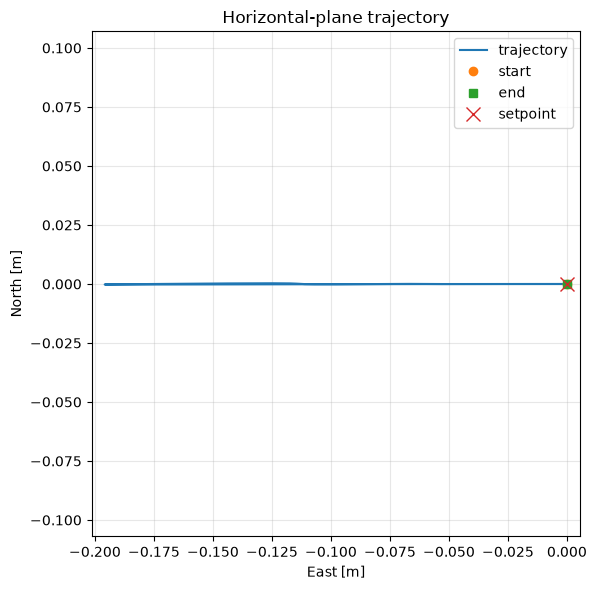
\includegraphics[width=0.48\linewidth]{figures/sim1a_xy.png}
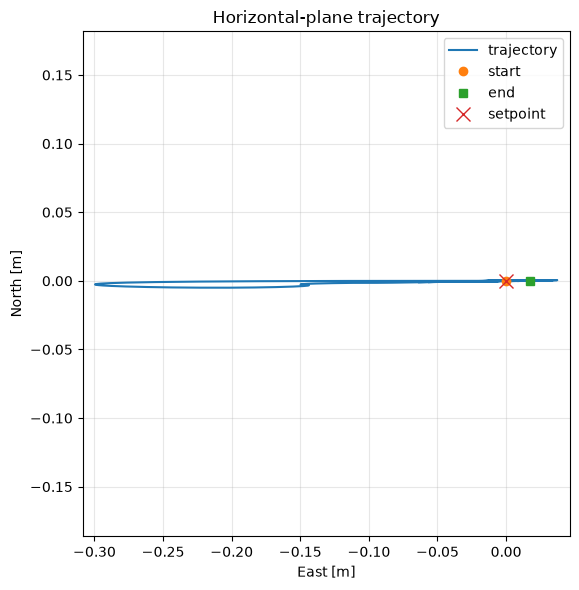
\includegraphics[width=0.48\linewidth]{figures/sim1b_xy.png}
\caption{Simulation 1 $xy$-trajectory: (a) current only (left), (b)
wind only (right).}
\label{fig:sim1-xy}
\end{figure}

\begin{figure*}[htbp]
\centering
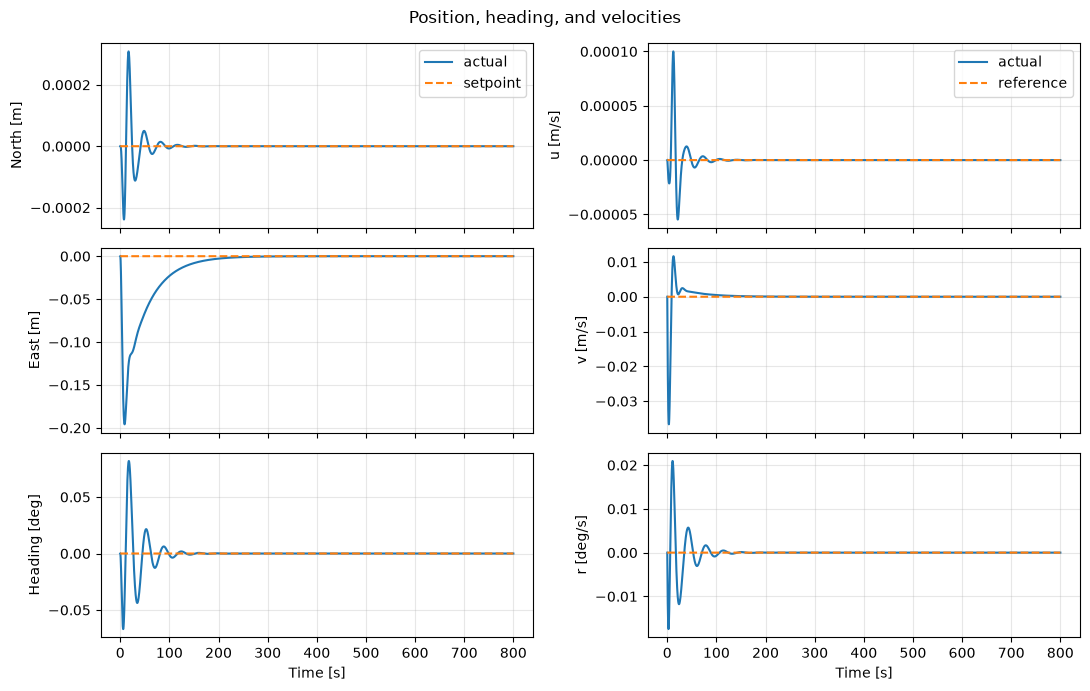
\includegraphics[width=0.48\linewidth]{figures/sim1a_time_histories.png}
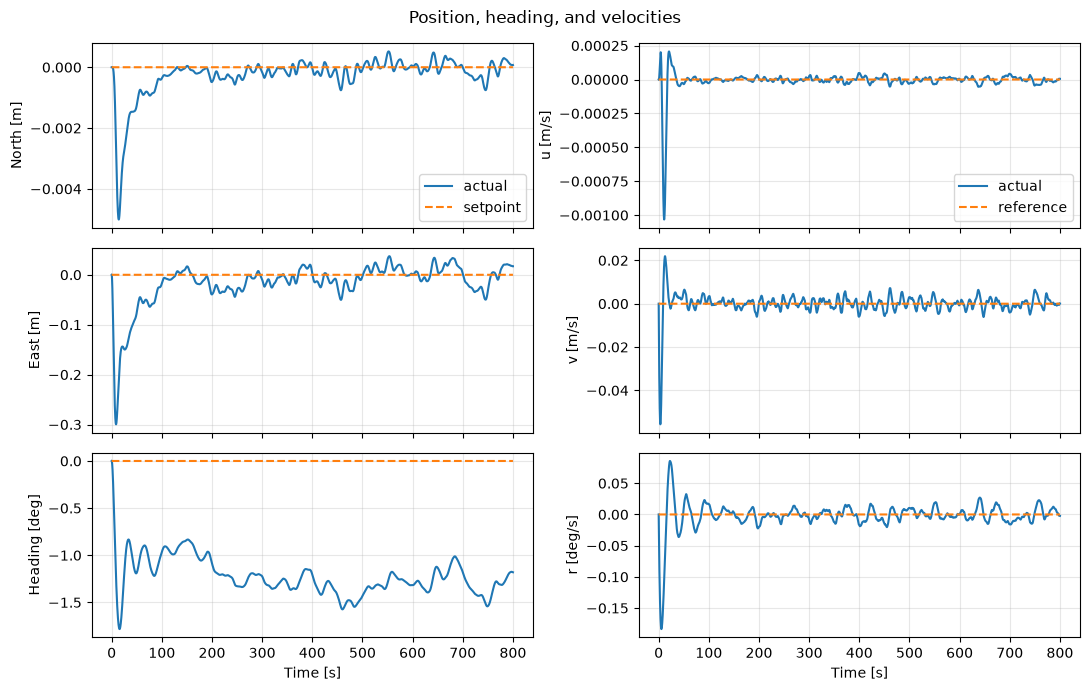
\includegraphics[width=0.48\linewidth]{figures/sim1b_time_histories.png}
\caption{Simulation 1 position, heading, and velocities vs.\ setpoint:
(a) current only (left), (b) wind only (right).}
\label{fig:sim1-time}
\end{figure*}

\begin{figure}[htbp]
\centering
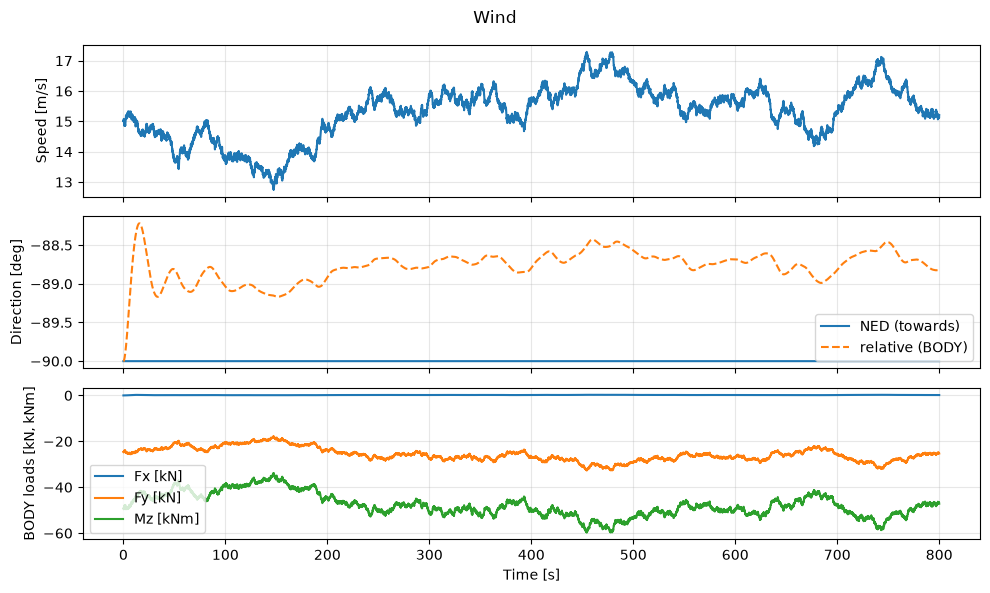
\includegraphics[width=\linewidth]{figures/sim1b_wind.png}
\caption{Simulation 1b: relative wind speed, direction, and body-frame
components driving the wind load.}
\label{fig:sim1b-wind}
\end{figure}

\begin{figure}[htbp]
\centering
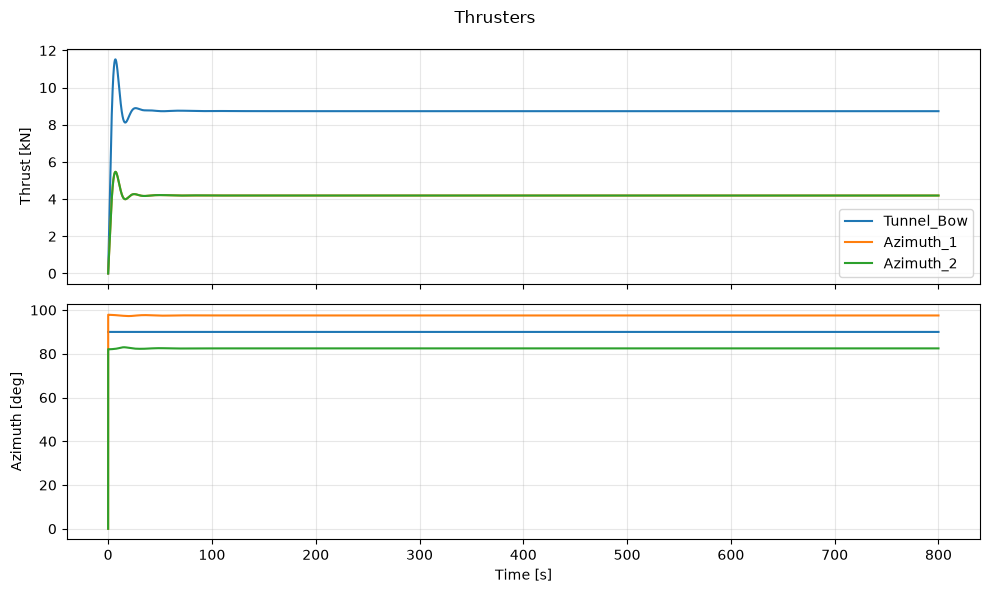
\includegraphics[width=0.48\linewidth]{figures/sim1a_thrusters.png}
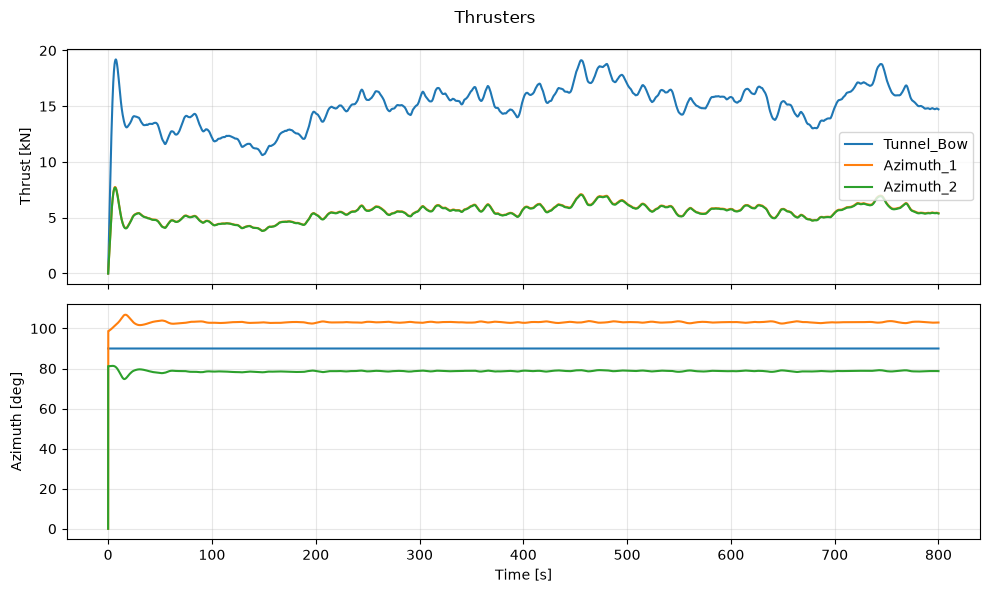
\includegraphics[width=0.48\linewidth]{figures/sim1b_thrusters.png}
\caption{Simulation 1 thruster effort: (a) current only (left), (b)
wind only (right). Both stay well within $u_{\max}$.}
\label{fig:sim1a-thrusters}
\label{fig:sim1b-thrusters}
\end{figure}

\todo{Report max/steady-state position error, settling time, and
actuator effort for each case using
Figs.~\ref{fig:sim1-xy}--\ref{fig:sim1a-thrusters} above.}

\subsection{Simulation 2: Rotating Current}
Current direction rotates linearly from north to east over 300 s at a
constant 0.5 m/s, no wind, vessel holding the origin.

\begin{figure}[htbp]
\centering
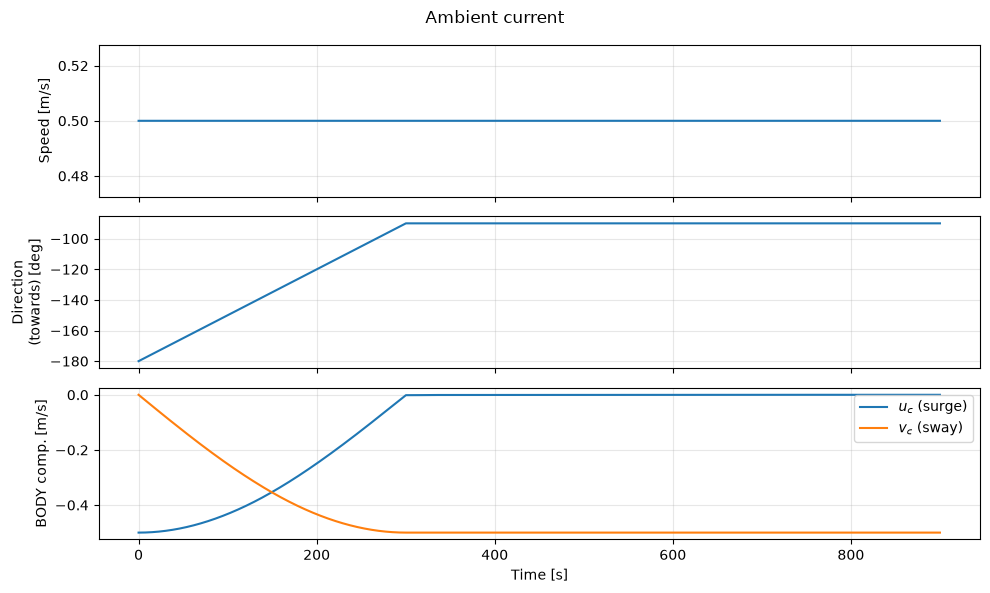
\includegraphics[width=\linewidth]{figures/sim2_current.png}
\caption{Simulation 2: ambient current speed, direction, and
body-frame components during the 300 s rotation.}
\label{fig:sim2-current}
\end{figure}

\begin{figure}[htbp]
\centering
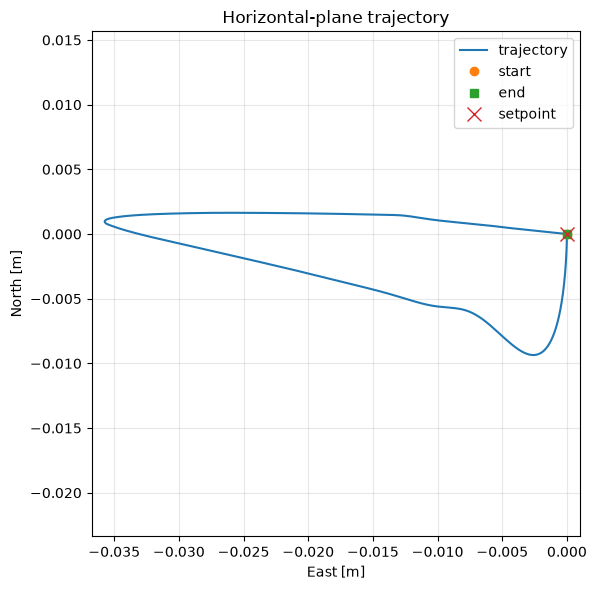
\includegraphics[width=0.48\linewidth]{figures/sim2_xy.png}
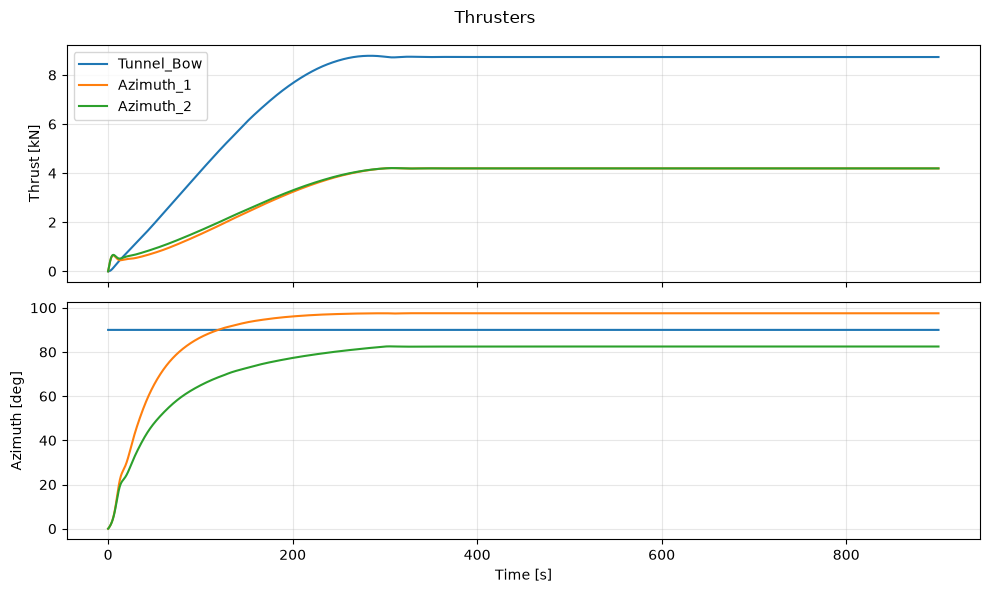
\includegraphics[width=0.48\linewidth]{figures/sim2_thrusters.png}
\caption{Simulation 2: $xy$-trajectory (left) and thruster commands
(right) during the current rotation.}
\label{fig:sim2-xy-thr}
\end{figure}

\todo{Discuss how the controller reacts during the 300 s rotation vs.\
behaviour once the current direction stabilises (see
Fig.~\ref{fig:sim2-current} for the current input and
Fig.~\ref{fig:sim2-xy-thr} for the resulting position hold /
actuator effort).}

\subsection{Simulation 3: Setpoint Change With and Without Reference Model}
\label{sec:sim3}
From $\eta_0=[0,0,0]^\top$ to $\eta_{sp}=[10,10,3\pi/2]^\top$, no
environmental forces, with and without the reference model. Since
$3\pi/2$ is equivalent to $-\pi/2$, the controller correctly turns
the vessel the short way: the logged heading converges to
$\psi\approx-\pi/2$ rather than completing an unnecessary $+3\pi/2$
rotation.

\begin{figure*}[htbp]
\centering
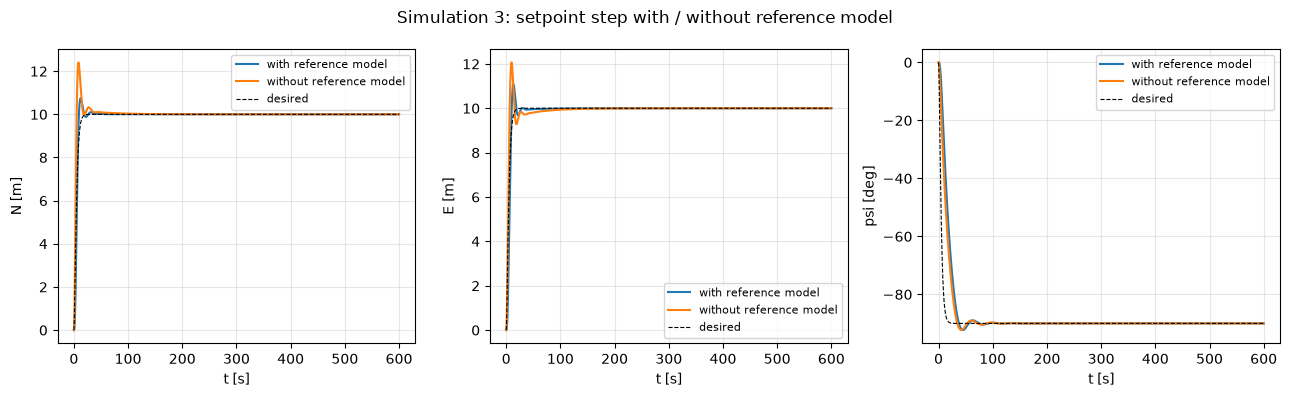
\includegraphics[width=0.9\linewidth]{figures/sim3_comparison.png}
\caption{Simulation 3: $N$, $E$, and $\psi$ with vs.\ without the
reference model, against the desired trajectory. Both runs converge
cleanly to the setpoint -- the pathology below is invisible at this
level.}
\label{fig:sim3-comparison}
\end{figure*}

\begin{figure}[htbp]
\centering
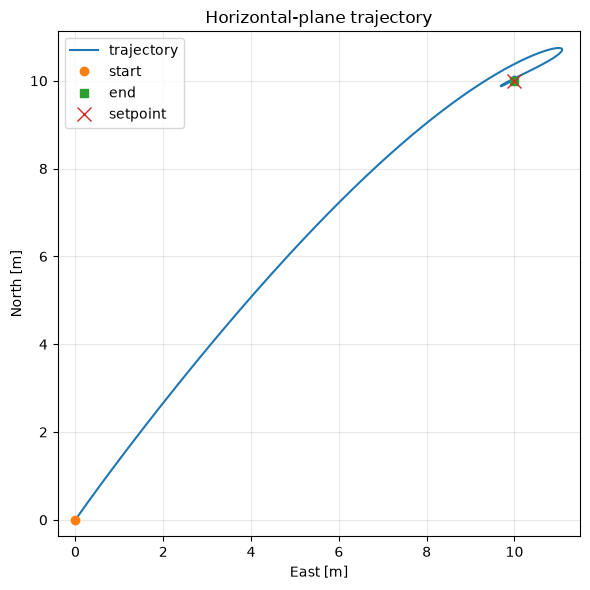
\includegraphics[width=0.48\linewidth]{figures/sim3_ref_xy.png}
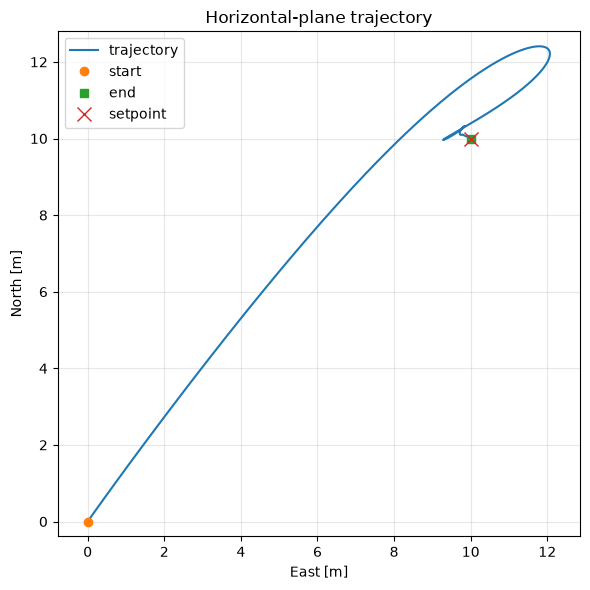
\includegraphics[width=0.48\linewidth]{figures/sim3_raw_xy.png}
\caption{Simulation 3 $xy$-trajectory: with reference model (left) vs.\
without (right).}
\label{fig:sim3-xy}
\end{figure}

\begin{figure}[htbp]
\centering
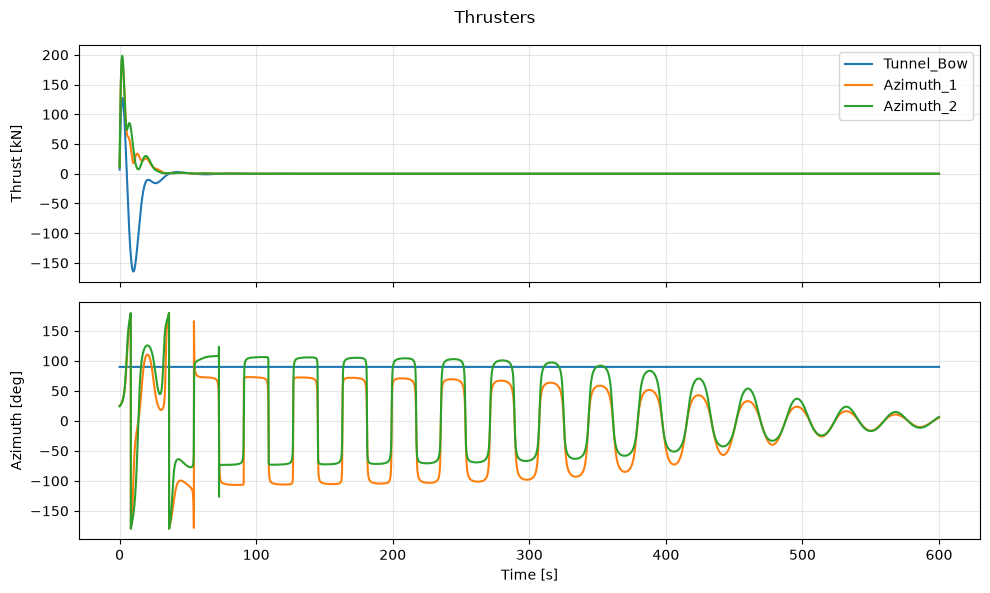
\includegraphics[width=\linewidth]{figures/sim3_ref_thrusters.png}
\caption{Simulation 3 (with reference model) thruster commands: an
initial spike to $\sim\!200\,\mathrm{kN}$ (vs.\ an 80 kN limit),
followed by a slowly-damping azimuth oscillation for the entire
600 s run -- invisible in Fig.~\ref{fig:sim3-comparison}, but not in
the underlying actuator commands.}
\label{fig:sim3-thrusters}
\end{figure}

Inspecting the per-thruster logs from this scenario (Fig.~\ref{fig:sim3-thrusters}) reveals a notable
allocator behaviour: both azimuth angles repeatedly swing by up to
$\sim\!160^\circ$ within a single $0.05\,\mathrm{s}$ time step (e.g.\
Azimuth\_1: $-97.5^\circ\!\to\!63.3^\circ$), with the two thrusters
flipping together rather than independently. Cross-referencing against
the commanded thrust magnitude at each jump shows $u_j\approx0$–$1\,
\mathrm{N}$ at exactly those instants -- i.e.\ the jumps occur when
the demanded force from that thruster passes through zero. The
demanded wrench during this phase is almost a pure yaw moment
$M_z(t)$ that oscillates in sign with slowly decaying amplitude (a
lightly damped closed-loop yaw oscillation), with negligible $F_x$,
$F_y$. Producing $+M_z$ or $-M_z$ with the stern azimuths requires
sideways force of opposite sign, i.e.\ thrust pointing at
$\alpha\approx+90^\circ$ or $\alpha\approx-90^\circ$. Because
Eq.~\eqref{eq:recover} always returns a non-negative magnitude, each
sign change of $M_z$ is represented as a discontinuous $\sim\!180^\circ$
azimuth flip rather than a smooth pass through zero thrust -- the
angle-ambiguity effect noted in Section~\ref{sec:alloc-limits}, where
$(u,\alpha)$ and $(-u,\alpha+\pi)$ produce the same force. The two
azimuths flip together because the symmetric layout
($y=\pm3\,\mathrm{m}$) makes the minimum-norm solution split the
demand almost equally between them, so both cross zero at the same
instant. The tunnel thruster is unaffected since its command is a
signed thrust at a fixed angle. Separately, the initial transient of
this scenario demands about $2.5\times$ the azimuth capacity
(Section~\ref{sec:alloc-limits}).

\todo{The initial oversized demand likely reflects controller tuning /
missing anti-windup (\S6.3) -- confirm with whoever owns the
controller section. Whether the sustained yaw oscillation is related
to that or is a separate lightly damped mode of the heading loop has
not been verified. The angle-flip behaviour itself is a property of
the allocator's representation of the force, not of the controller.
Insert the with vs.\ without reference model thruster plots here once
finalised.}

\subsection{Simulation 4: Four-Corner Test}
Setpoints $\eta_0,\ldots,\eta_5$ from Table~2 of the project text,
300 s hold per corner, no environmental forces.

\begin{figure*}[htbp]
\centering
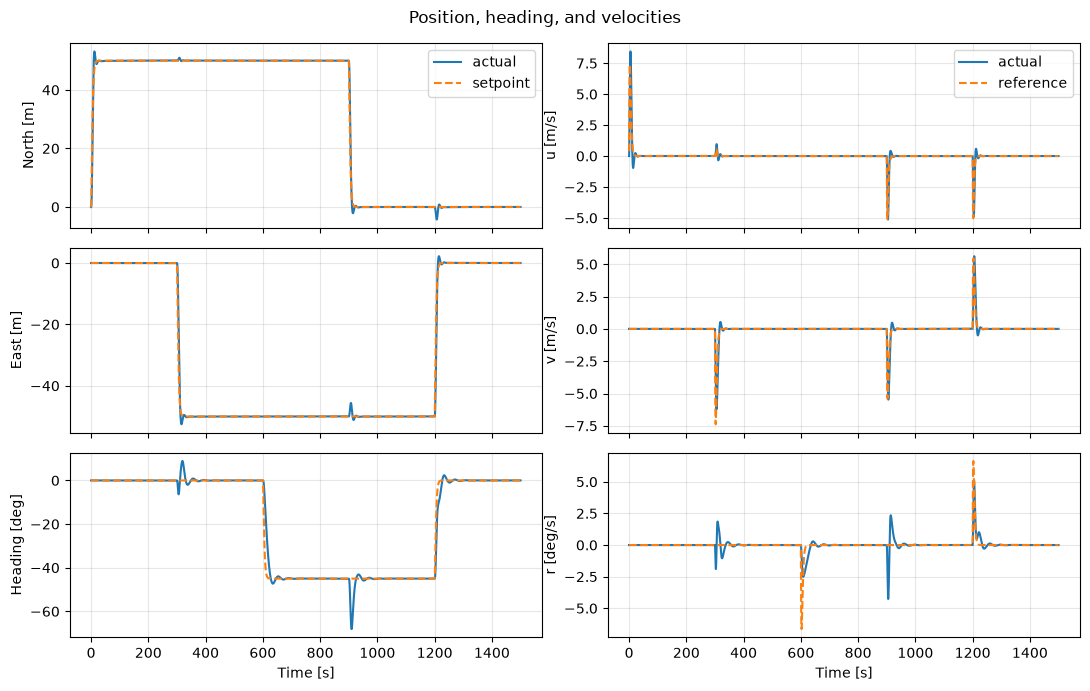
\includegraphics[width=0.48\linewidth]{figures/sim4_time_histories.png}
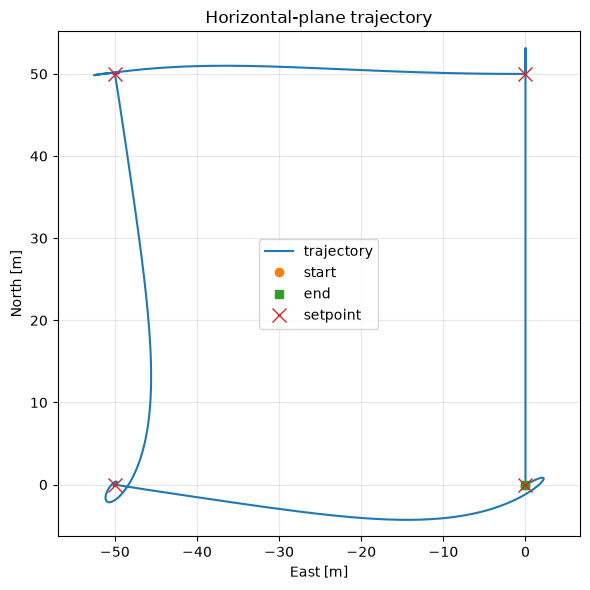
\includegraphics[width=0.48\linewidth]{figures/sim4_xy.png}
\caption{Simulation 4 (four-corner test): position, heading, and
velocities vs.\ setpoint (left); $xy$-trajectory through all five
corners (right).}
\label{fig:sim4}
\end{figure*}

\begin{figure}[htbp]
\centering
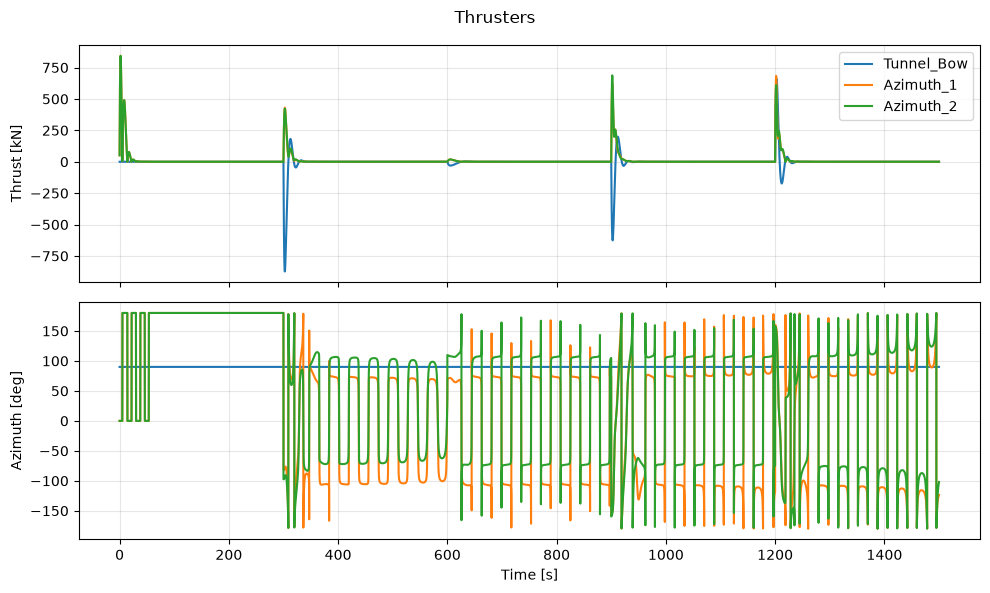
\includegraphics[width=\linewidth]{figures/sim4_thrusters.png}
\caption{Simulation 4 thruster commands across all five corners.}
\label{fig:sim4-thrusters}
\end{figure}

\todo{Verify and discuss whether the vessel reaches steady position
before each transition (Fig.~\ref{fig:sim4}), and check whether the
same azimuth-flip pathology from Simulation 3
(Fig.~\ref{fig:sim3-thrusters}) reappears here at larger, sustained
setpoint changes (Fig.~\ref{fig:sim4-thrusters}).}

\section*{Individual Contributions}
The wind and current models were written entirely by an AI assistant
(Google, Gemini), because the group member originally assigned to
them left the group. \todo{Add the factual, specific contribution of
each remaining group member.}

\section*{Acknowledgment}
\todo{Remove this section, or use it if relevant.}

\begin{thebibliography}{1}
\bibitem{fossen2011}
T.~I. Fossen, \emph{Handbook of Marine Craft Hydrodynamics and Motion
Control}. Chichester, UK: Wiley, 2011.
\bibitem{blendermann1994}
W.~Blendermann, ``Parameter identification of wind loads on ships,''
\emph{Journal of Wind Engineering and Industrial Aerodynamics},
vol.~51, no.~3, pp.~339--351, 1994.
\end{thebibliography}

\end{document}
